\documentclass{beamer}
\usetheme{default}

\usepackage{graphicx}
\usepackage{hyperref} 
\graphicspath{{../../images/}}

\setbeamertemplate{caption}[numbered]

\title{Chapter-11: Orchestration-driven Service-oriented Architecture}
\subtitle{IF231303-Software Architecture\\Pradita University}
\author{Hansel Ricardo, Jonathan Erik Maruli Tua, Yefta Tanuwijaya}
\begin{document}
	
	\begin{frame}[plain]
		\maketitle
	\end{frame}
	
	\begin{frame}{DevOps}
		\begin{figure}[h]
			\centering
			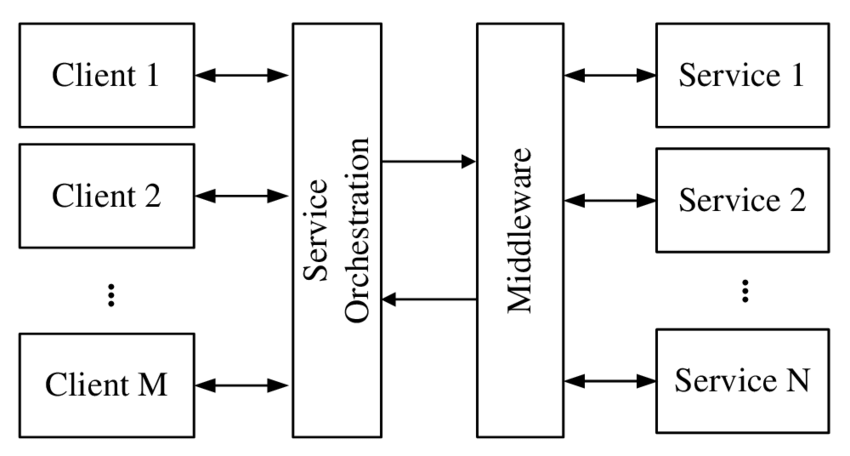
\includegraphics[width=\textwidth]{ODSOA}
			\caption{Arsitektur ODSOA.}
			\label{fig:Arsitektur ODSOA}
		\end{figure}
	\end{frame}
	
	\begin{frame}{Latar Belakang}
		\begin{itemize}
			\item Pengertian
			\\\textit{Orchestration-driven Service-oriented Architecture} (ODSOA) adalah suatu pendekatan arsitektur perangkat lunak yang bertujuan untuk memfasilitasi pengembangan dan integrasi sistem yang kompleks dengan cara menggunakan layanan (\textit{Services}) yang terdistribusi dan terpisah secara fisik namun saling terkait secara fungsional.
		\end{itemize}
	\end{frame}
	
	\begin{frame}{Komponen}
		Komponen utama dalam \textit{Orchestration-driven Service-oriented Architecture} (ODSOA) antara lain:
		\begin{itemize}
			\item Layanan (\textit{Services})
			\item Orkestrasi (\textit{Orchestration})
			\item Bus Layanan (\textit{Service Bus})
			\item Repositori Layanan (\textit{Service Repository})
			\item Klien (\textit{Client})
			\item Penyedia Layanan (\textit{Service Provider})
			
		\end{itemize}
	\end{frame}
	
	\begin{frame}{Kelebihan}
		Kelebihan dari mengimplementasikan \textit{Orchestration-driven Service-oriented Architecture} (ODSOA) adalah:
		\begin{itemize}
			\item Layanan dapat dikonfigurasi ulang atau ditambahkan ke infrastruktur dengan mudah, tanpa mempengaruhi sistem keseluruhan.
			\item Memodifikasi fungsionalitas sistem dan mengintegrasikan solusi baru tanpa mempengaruhi sistem keseluruhan.
			\item Berintegrasi dengan sistem lain dengan mudah dan memperluas fungsionalitas sistem mereka.
			\item Dapat digunakan kembali oleh aplikasi dan sistem lain.
			\item Memisahkan tugas-tugas sistem menjadi layanan yang terpisah secara fisik namun saling terkait secara fungsional.
			
		\end{itemize}
	\end{frame}
	
	\begin{frame}{Kekurangan}
		Kekurangan dari mengimplementasikan \textit{Orchestration-driven Service-oriented Architecture} (ODSOA) adalah:
		\begin{itemize}
			\item Dapat menjadi sangat kompleks ketika aplikasi memiliki banyak layanan.
			\item Memerlukan tingkat keahlian teknis yang tinggi untuk mengimplementasikan dan mengelola arsitektur ini dengan efektif.
			\item Melibatkan layanan dari banyak sistem dan vendor, sehingga keamanannya harus selalu diperhatikan.
			\item Implementasi arsitektur ODSOA memerlukan biaya yang tinggi karena melibatkan pengembangan, integrasi, dan manajemen layanan yang kompleks.
			\item Bergantung pada vendor tertentu untuk memasok layanan tertentu.
			\item Perubahan pada satu layanan dapat mempengaruhi layanan lainnya.
		\end{itemize}
	\end{frame}
	
	\begin{frame}{Contoh Kasus}
		\begin{itemize}
			\item Dengan menggunakan Python, menyelesaikan sebuah masalah pengecekan umur untuk membuat KTP.
			\item Dimulai dari verifikasi data diri, dan mengecek apakah umurnya sudah cukup untuk membuat KTP.
			%\text Glenny: begin itemize dulu ya
		\end{itemize}
	\end{frame}
	
\end{document}